\chapter{Introducción General}

\label{Capitulo1}

\newcommand{\keyword}[1]{\textbf{#1}}
\newcommand{\tabhead}[1]{\textbf{#1}}
\newcommand{\code}[1]{\texttt{#1}}
\newcommand{\file}[1]{\texttt{\bfseries#1}}
\newcommand{\option}[1]{\texttt{\itshape#1}}
\newcommand{\grados}{$^{\circ}$}

En este capítulo se introduce al campo de estudio de la robótica móvil. Se aborda una comparativa entre diferentes plataformas didácticas comerciales y se exponen el alcance y las motivaciones que llevaron al desarrollo del presente proyecto.

\section{Robótica móvil}

La robótica móvil se encarga del estudio de los robots móviles, haciendo especial hincapié en el desarrollo de capacidades permitan a lo mismos, decidir de manera autónoma cómo, cuándo y a dónde moverse.\newline
En contraste con los robots manipuladores cuya base se encuentra fija con respecto a un sistema de referencia, los robots móviles son aquellos capaces de moverse a si mismos de un lugar a otro. Esta particularidad obliga a que los robots móviles deban ser capaces de interactuar con entornos no determinísticos, es decir, propensos a situaciones impredecibles como por ejemplo, una puerta entreabierta, un objeto o persona obstaculizando el camino, etc.\newline

\subsection{Tipos de robots móviles}

Dependiendo de cómo realizan su locomoción, es posible caracterizar a los robots móviles en los siguientes tipos:
\begin{itemize}
	\item{Robots con patas}
	\item{Robots aéreos}
	\item{Robots con ruedas}
\end{itemize}

Cada uno de estos tipos plantea su propio set de ventajas y desventajas, así como dificultades para su implementación. En el presente trabajo se hará énfasis solo en el último tipo de la lista, es decir en robots con ruedas.

\newpage

\section{Estado del arte}

Existe una amplia gama de robots móviles con ruedas ofrecidos específicamente para el sector académico. A continuación se ofrece un breve sumario de opciones que se encuentran actualmente en el mercado.
\subsection{TurtleBot}

TurtleBot constituye al día de hoy una familia de robots móviles para uso personal de bajo costo. Su uso se extiende tanto a la academia como a roboticistas aficionados en todo el mundo.\newline
Aunque su primera iteración vió la luz en 2010 con un set de características bastante modestas, el lanzamiento de nuevas versiones le aseguró su lugar como dispositivo de referencia para la plataforma ROS. \newline
Muchas de las consideraciones de diseño del robot propuesto en este trabajo fueron del turtlebot 2, mostrado en la figura \ref{fig:robotTurtlebot}.

\begin{figure}[ht]
	\centering
	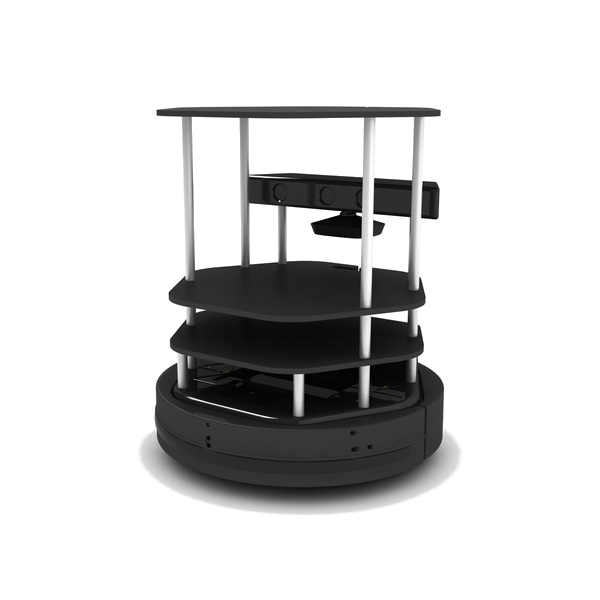
\includegraphics[scale=1.5]{./Figures/turtlebot.png}
	\caption{Vista frontal del turtlebot 2 con un sensor Kinect acoplado.\protect\footnotemark}
	\label{fig:robotTurtlebot}
\end{figure}

\footnotetext{\url{https://img.directindustry.es/images_di/photo-g/177123-10073681.jpg}}

\subsection{Clearpath Jackal}

El Jackal es un robot móvil 4x4 apto para uso en exteriores. Su robustez lo hacen la elección preferida de muchas universidades a la hora de implementar soluciones "de campo", principalmente debido a su resistencia total al polvo y al agua de lluvia.\newline
Posee una capacidad de carga de hasta 20 kg, lo que lo hace apto para cargar una importante cantidad de sensores, actuadores y manipuladores, tal como el ejemplo mostrado en la figura \ref{fig:robotJackal}.

\begin{figure}[ht]
	\centering
	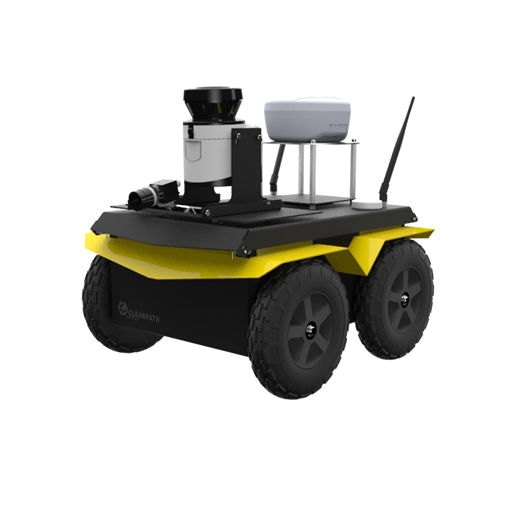
\includegraphics[scale=1.6]{./Figures/jackal.png}
	\caption{Vista frontal de la base robótica Jackal con una batería de sensores instalados por el usuario.\protect\footnotemark}
	\label{fig:robotJackal}
\end{figure}

\footnotetext{\url{https://img.directindustry.es/images_di/photo-g/177123-10073681.jpg}}

\subsection{Fetch Freight 100 Base}

Fetch Robotics ofrece con el Freight 100 Base una base robótica para uso en interiores \citep{PAPER:1}. La misma fue diseñada específicamente para moverse en edificios adaptados a personas en sillas de ruedas que cumplen con la normativa ADA o \textit{Americans with Disabilities Act}.\newline
El Freight 100 incluye un sensor del tipo LIDaR 2D, mostrado en la figura \ref{fig:robotFreight}, lo que lo hace adecuado para tareas de navegación. Además, al estar basado en un robot industrial de carga, la base Freight 100 esta diseñada para soportar la impresionante cantidad de hasta 100 kg de peso, por lo que puede cargar con un manipulador industrial en su lomo.

\begin{figure}[ht]
	\centering
	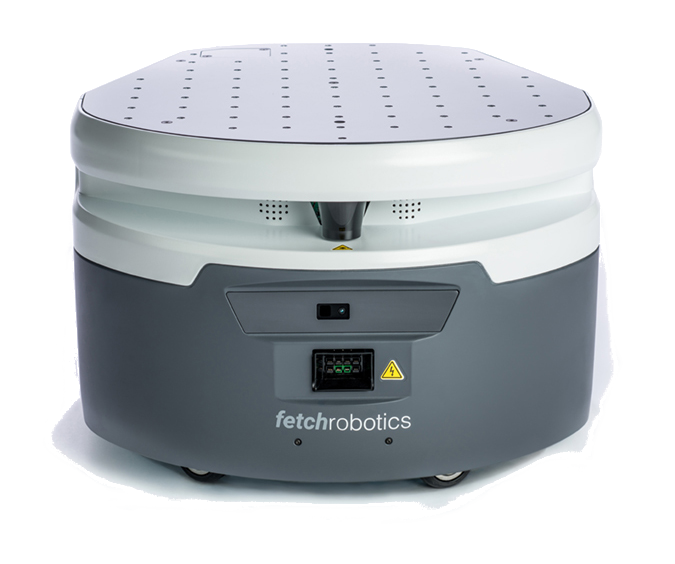
\includegraphics[scale=1.0]{./Figures/freight.png}
	\caption{Vista frontal de la base robótica Fetch Freight donde se puede apreciar su sensor integrado del tipo LIDaR.\protect\footnotemark}
	\label{fig:robotFreight}
\end{figure}

\footnotetext{\url{https://www.dymesich.com/wp-content/uploads/2019/06/freight-100-low.jpg}}

\subsection{FESTO Robotino}

Robotino es un robot móbil comercializado por la compañía alemana FESTO Didactic. El mismo esta diseñado para entornos educativos, de entrenamiento y de investigación.
Esta plataforma dispone de un sistema de tracción omni que como su nombre sugiere, le otorga libertad de movimiento omnidireccional en dos dimensiones.\newline
Asímismo, Robotino viene equipado de fábrica con una computadora tipo PC de grado industrial, lo que facilita su integración con elementos de hardware y software externos tales como cámaras, sensores y actuadores que utilicen el protocolo RS-232, RS-485 o USB. En la figura \ref{fig:robotRobotino} se puede apreciar una webcam acoplada al mismo.

\begin{figure}[ht]
	\centering
	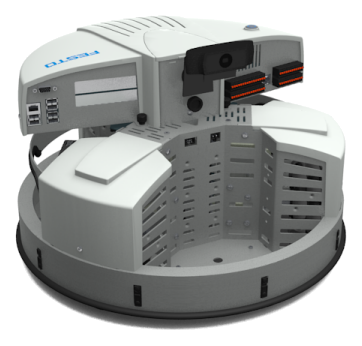
\includegraphics[scale=1.4]{./Figures/robotino.png}
	\caption{Vista frontal del Robot FESTO Robotino con una webcam acoplada al mismo.\protect\footnotemark}
	\label{fig:robotRobotino}
\end{figure}

\footnotetext{\url{https://www.festo-didactic.com/ov3/media/customers/1100/robotinohome.png}}


\subsection{Pioneer 3-DX}

El Pioneer 3-DX es un pequeño robot de tracción diferencial ideal para utilizarse en entornos académicos ya sea de laboratorio o en salón de clases. El mismo incorpora de fábrica cinco sensores del tipo Sonar al frente del robot como los que se pueden apreciar en la figura \ref{fig:robotPioneer}, encoders para las ruedas y un microcontrolador con firmware específico.\newline
Su amplia superficie de carga le permite mover cargas de hasta 8 Kg, por lo que es un buen candidato para añadir sensores y actuadores extra, como cámaras o manipuladores.

\begin{figure}[ht]
	\centering
	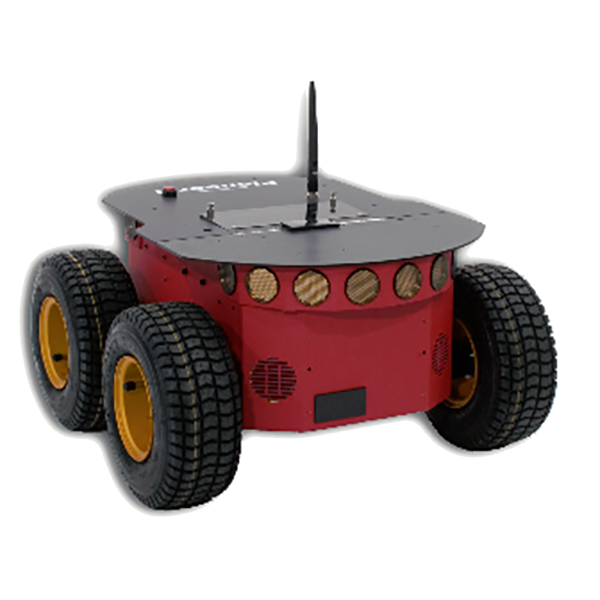
\includegraphics[scale=1.]{./Figures/pioneer.png}
	\caption{Vista frontal del Robot Pioneer donde se aprecian sus cinco sensores sonar.\protect\footnotemark}
	\label{fig:robotPioneer}
\end{figure}

\footnotetext{\url{https://static.generation-robots.com/6645-large_default/robot-mobile-pioneer-3-at.jpg}}


\section{Motivación}

Los robots móviles expuestos en la sección anterior representan propuestas comerciales listas para usar que permiten a profesores, investigadores y alumnos concentrarse en el estudio o desarrollo de aplicaciones de la robótica móvil, eliminando la necesidad de diseñar un robot desde cero para cada caso de uso específico. Gracias a esto, las instituciones o individuos que adquieren dichos equipos pueden concentrarse de inmediato en las tareas de interés para el estudio de la materia, ahorrando tiempo y esfuerzo.\newline
Resulta tentador entonces preguntarse ¿por qué no todas las instituciones adquieren un robot comercial para el laboratorio de robótica?. La respuesta esta en los altos costos asociados a la adquisición de estos equipos. Los robots destinados a investigación son costosos y por ende, son pocas las instituciones educativas en condiciones de invertir en ellos.


\section{Objetivos}

Mediante este trabajo se propone una plataforma destinada a la enseñanza de robótica móvil en instituciones educativas de nivel universitario de código abierto y con componentes disponibles en el mercado local argentino.

\section{Alcance}

Se procedió a separar el alcance en base al tipo de trabajo realizado, así como lo que no se incluye con el mismo.

El alcance del presente trabajo involucró el desarrollo del firmware para el microcontrolador encargado de:
\begin{itemize}
	\item Intermediar la comunicación entre la base robótica ``Roomba 500'' y el framework de robótica ROS (\textit{Robot Operating System}).
	\item Realizar la interfaz entre la unidad de medición inercial MPU6050 con ROS.
	\item Port de la librería rosserial para ser utilizada con FreeRTOS y STM32Cube HAL en el lenguaje de programación C++.
\end{itemize}

Se incluye el desarrollo de softwere requerido para:
\begin{itemize}
	\item El paquete para ROS que brinda soporte básico para el robot propuesto "Lubobot", con sus sensores y actuadores.
	\item Calcular la odometría del robot utilizando las lecturas de los encoders.
	\item La descripción del robot en formato URDF (\textit{Unified Robot Description Format}), requerido para representar correctamente el robot en la herramienta RViz.
	\item Una imagen de Docker con todas las dependencias necesarias para utilizar el robot de manera encapsulada y sin la necesidad de modificar la configuración del sistema operativo del usuario.
\end{itemize}

Se incluye una seccion extra en el repositorio oficial en GitHub con una Wiki con la documentación básica necesaria para que un nuevo usuario sea capaz de:

\begin{itemize}
	\item Armar un nuevo robot idéntico al propuesto.
	\item Configurar el robot para utilizar el stack de navegación de ROS.
\end{itemize} 

No se incluye con el presente trabajo:
\begin{itemize}
	\item Ningún algoritmo de navegación local ni global.
	\item Código requerido para la conexión al microcontrolador mediante Ethernet.
\end{itemize}